\documentclass[tikz,border=10pt]{standalone}
\begin{document}
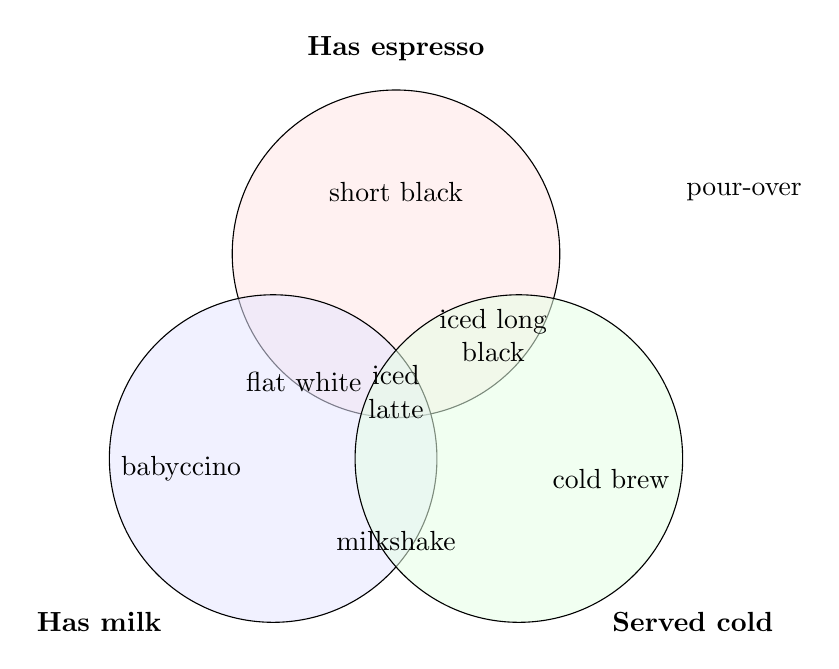
\begin{tikzpicture}[scale=1.3]
  \def\r{1.6}
  \coordinate (A) at (0,1.2);    % espresso
  \coordinate (B) at (-1.2,-0.8);% milk
  \coordinate (C) at (1.2,-0.8); % cold

  \draw[fill=red!10,  fill opacity=0.55] (A) circle (\r);
  \draw[fill=blue!10, fill opacity=0.55] (B) circle (\r);
  \draw[fill=green!10,fill opacity=0.55] (C) circle (\r);

  % Labels
  \node[font=\bfseries] at (0,3.2) {Has espresso};
  \node[font=\bfseries] at (-2.9,-2.4) {Has milk};
  \node[font=\bfseries] at (2.9,-2.4) {Served cold};

  % espresso only
  \node at (0,1.8) {short black};
  % espresso + cold
  \node[align=center] at (0.95,0.4) {iced long\\black};
  % espresso + milk
  \node at (-0.9,-0.05) {flat white};
  % espresso + milk + cold
  \node[align=center] at (0,-0.15) {iced\\latte};
  % milk only
  \node at (-2.1,-0.9) {babyccino};
  % milk + cold
  \node at (0,-1.6) {milkshake};
  % cold only
  \node at (2.1,-1.0) {cold brew};
  % none
  \node at (3.4,1.8) {pour-over};
\end{tikzpicture}
\end{document}
